\documentclass{article}

% Language setting
% Replace `english' with e.g. `spanish' to change the document language
\usepackage{biblatex} %Imports biblatex package
\addbibresource{../Lab2/refs.bib}
\usepackage{enumitem}
\usepackage[english]{babel}
\usepackage{array}
\usepackage{amsmath}
\usepackage{pythonhighlight}
\usepackage{multirow}
\newcolumntype{P}[1]{>{\centering\arraybackslash}p{#1}}
\newcolumntype{M}[1]{>{\centering\arraybackslash}m{#1}}

% Set page size and margins
% Replace `letterpaper' with `a4paper' for UK/EU standard size
\usepackage[letterpaper,top=2cm,bottom=2cm,left=3cm,right=3cm,marginparwidth=1.75cm]{geometry}

\usepackage{amsmath}
\usepackage{graphicx}
\usepackage{caption}
\usepackage{subcaption}
\usepackage[colorlinks=true, allcolors=blue]{hyperref}
\usepackage{setspace}
\usepackage{booktabs}
\usepackage[T1]{fontenc}
\usepackage{longtable}
\doublespacing

\begin{document}
\newcommand{\Fig}[3]{\begin{figure}[!h!]\centering\includegraphics[width=0.5\linewidth]{#1}\caption{#2}\label{#3}\end{figure}}
\begin{titlepage}

\centering
\scshape
\vspace{\baselineskip}

%
\rule{\textwidth}{1.6pt}\vspace*{-\baselineskip}\vspace*{2pt}
\rule{\textwidth}{0.4pt}

{\Huge \textbf{\textsc{ Heat Treatment of Steels \\
\vspace{15pt}}}}

\rule{\textwidth}{0.4pt}\vspace*{-\baselineskip}\vspace{3.2pt}
\rule{\textwidth}{1.6pt}\vspace{6pt}
\centerline{\textit{University of Illinois at Urbana-Champaign}} 
\centerline{\textit{Department of Nuclear, Plasma, and Radiological Engineering}}
\vspace{1.5\baselineskip}


\large \centerline{\textbf{Author:} Nathan Glaser}
\large \centerline{\textbf{Net-ID:} nglaser3}
\quad

\vfill
\large \centerline{October 23, 2024}
%
\pagenumbering{gobble}
\end{titlepage}

\tableofcontents
\newpage
\pagenumbering{arabic}

\section{Abstract}

\section{Introduction}

\section{Experimental Methods}

\section{Theoretical Models}
\begin{equation}
    \textbf{H}_{BN} = 131.7 e^{0.0252\:\textbf{H}_{RC}}
    \label{eq:rc2br}
\end{equation}

\newpage
\section{Results}
To begin, we found the engineering stress-strain curves for oil quenched, water quenched, normalized, annealed, and oil quenched and tempered at both 300 and 500 $^oC$. 

\begin{figure}[!h!]
    \centering
    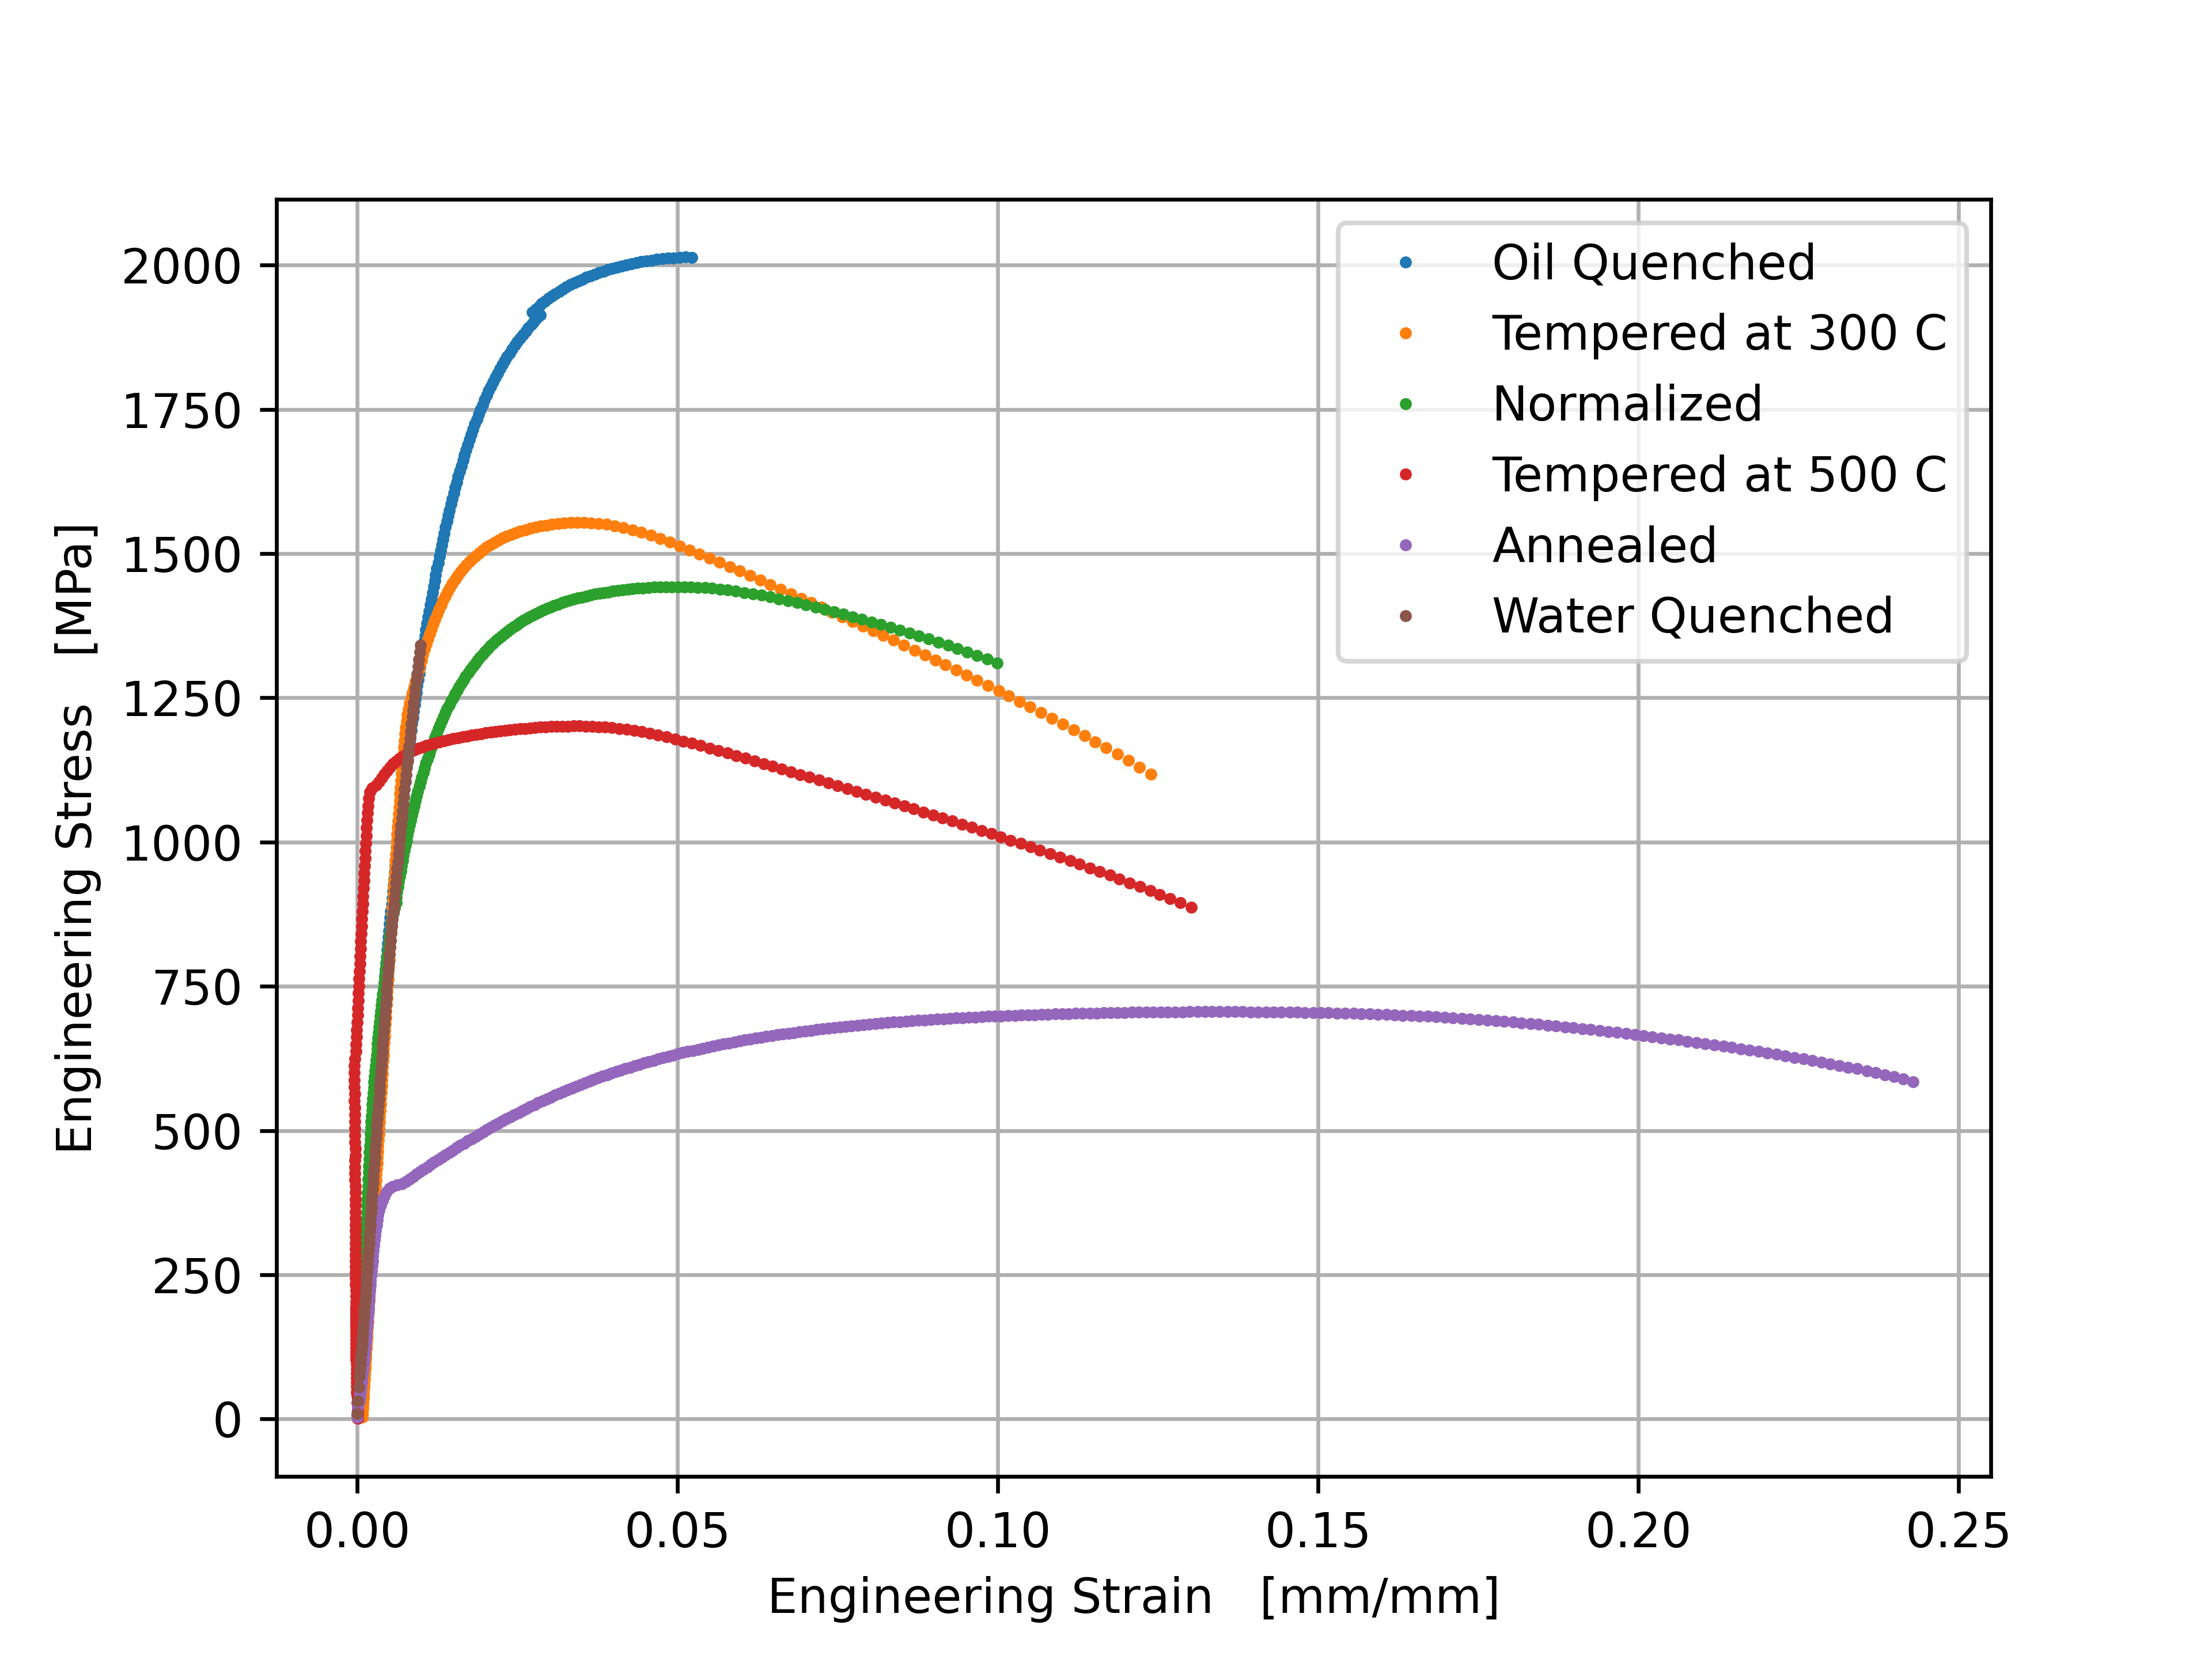
\includegraphics[width=0.5\linewidth]{Lab5/plots/q1_adjusted.png}
    \caption{Engineering Stress-Strain curves of select materials}
    \label{fig:q1-all}
\end{figure}

Next, from Fig. \ref{fig:q1-all} we found the elastic modulus, the yield strength, the ultimate strength, the toughness, percent elongation, and brinnel hardness for each specimen. To not have an overly wide table, the specimen names were abbreviated but follow the same order as in the legend of Fig. \ref{fig:q1-all}. The brinnel hardness values were determined via the conversionary equation, Eq. \ref{eq:rc2br}. The yield strengths were determined via the 0.2 \% offset methodology.

\begin{table}[!h!]
    \centering
    \renewcommand{\arraystretch}{1.5}
    \caption{Select material properties of each specimen tested}
    \begin{tabular}{|c|c|c|c|c|c|c|}
        \toprule
        \textbf{Material} & \textbf{OQ} & \textbf{Temp. 300} & \textbf{Norm.} & \textbf{Temp. 500} & \textbf{An.} & \textbf{WQ} \\ 
        \midrule
        \hline 
        \textbf{Youngs Modulus [GPa]} & 197.065 & 186.829 & 205.729 & 227.167 & 111.797 & 161.711 \\ 
        \hline 
        \textbf{Yield Strength} & 1138.428 & 1269.068 & 931.842 & 1148.958 & 402.874 & 1341.104 \\ 
        \hline 
        \textbf{Ultimate Strength} & 2013.803 & 1553.692 & 1442.464 & 1201.172 & 705.882 & 1341.104 \\ 
        \hline 
        \textbf{Toughness} & 86.562 & 166.139 & 131.696 & 142.251 & 155.675 & 7.386 \\ 
        \hline 
        \textbf{Percent Elongation} & 5.22 & 12.392 & 9.992 & 13.061 & 24.284 & 0.991 \\ 
        \hline 
        \textbf{Brinnel Hardness} & 264.692 & 309.453 & 238.109 & 247.905 & 1206.654 & 353.671 \\ 
        \hline 
    \end{tabular}
    \label{tab:q2}
\end{table}

Next, from these tabulated values we can determine a correlation between the  the ultimate strength and Brinnel hardness of each specimen, presented in Fig. \ref{fig:q4}. The linear-regression was performed with the use of \texttt{scipy.stats.linregress}. Next, again from Table \ref{tab:q2}, we determined the correlations between the ultimate strength, the yield strength, the elastic modulus, and the percent of elongation and the Brinnel hardness for specifically the oil quenched and the oil quenched then tempered specimens.

\begin{figure}[!h!]
    \centering
    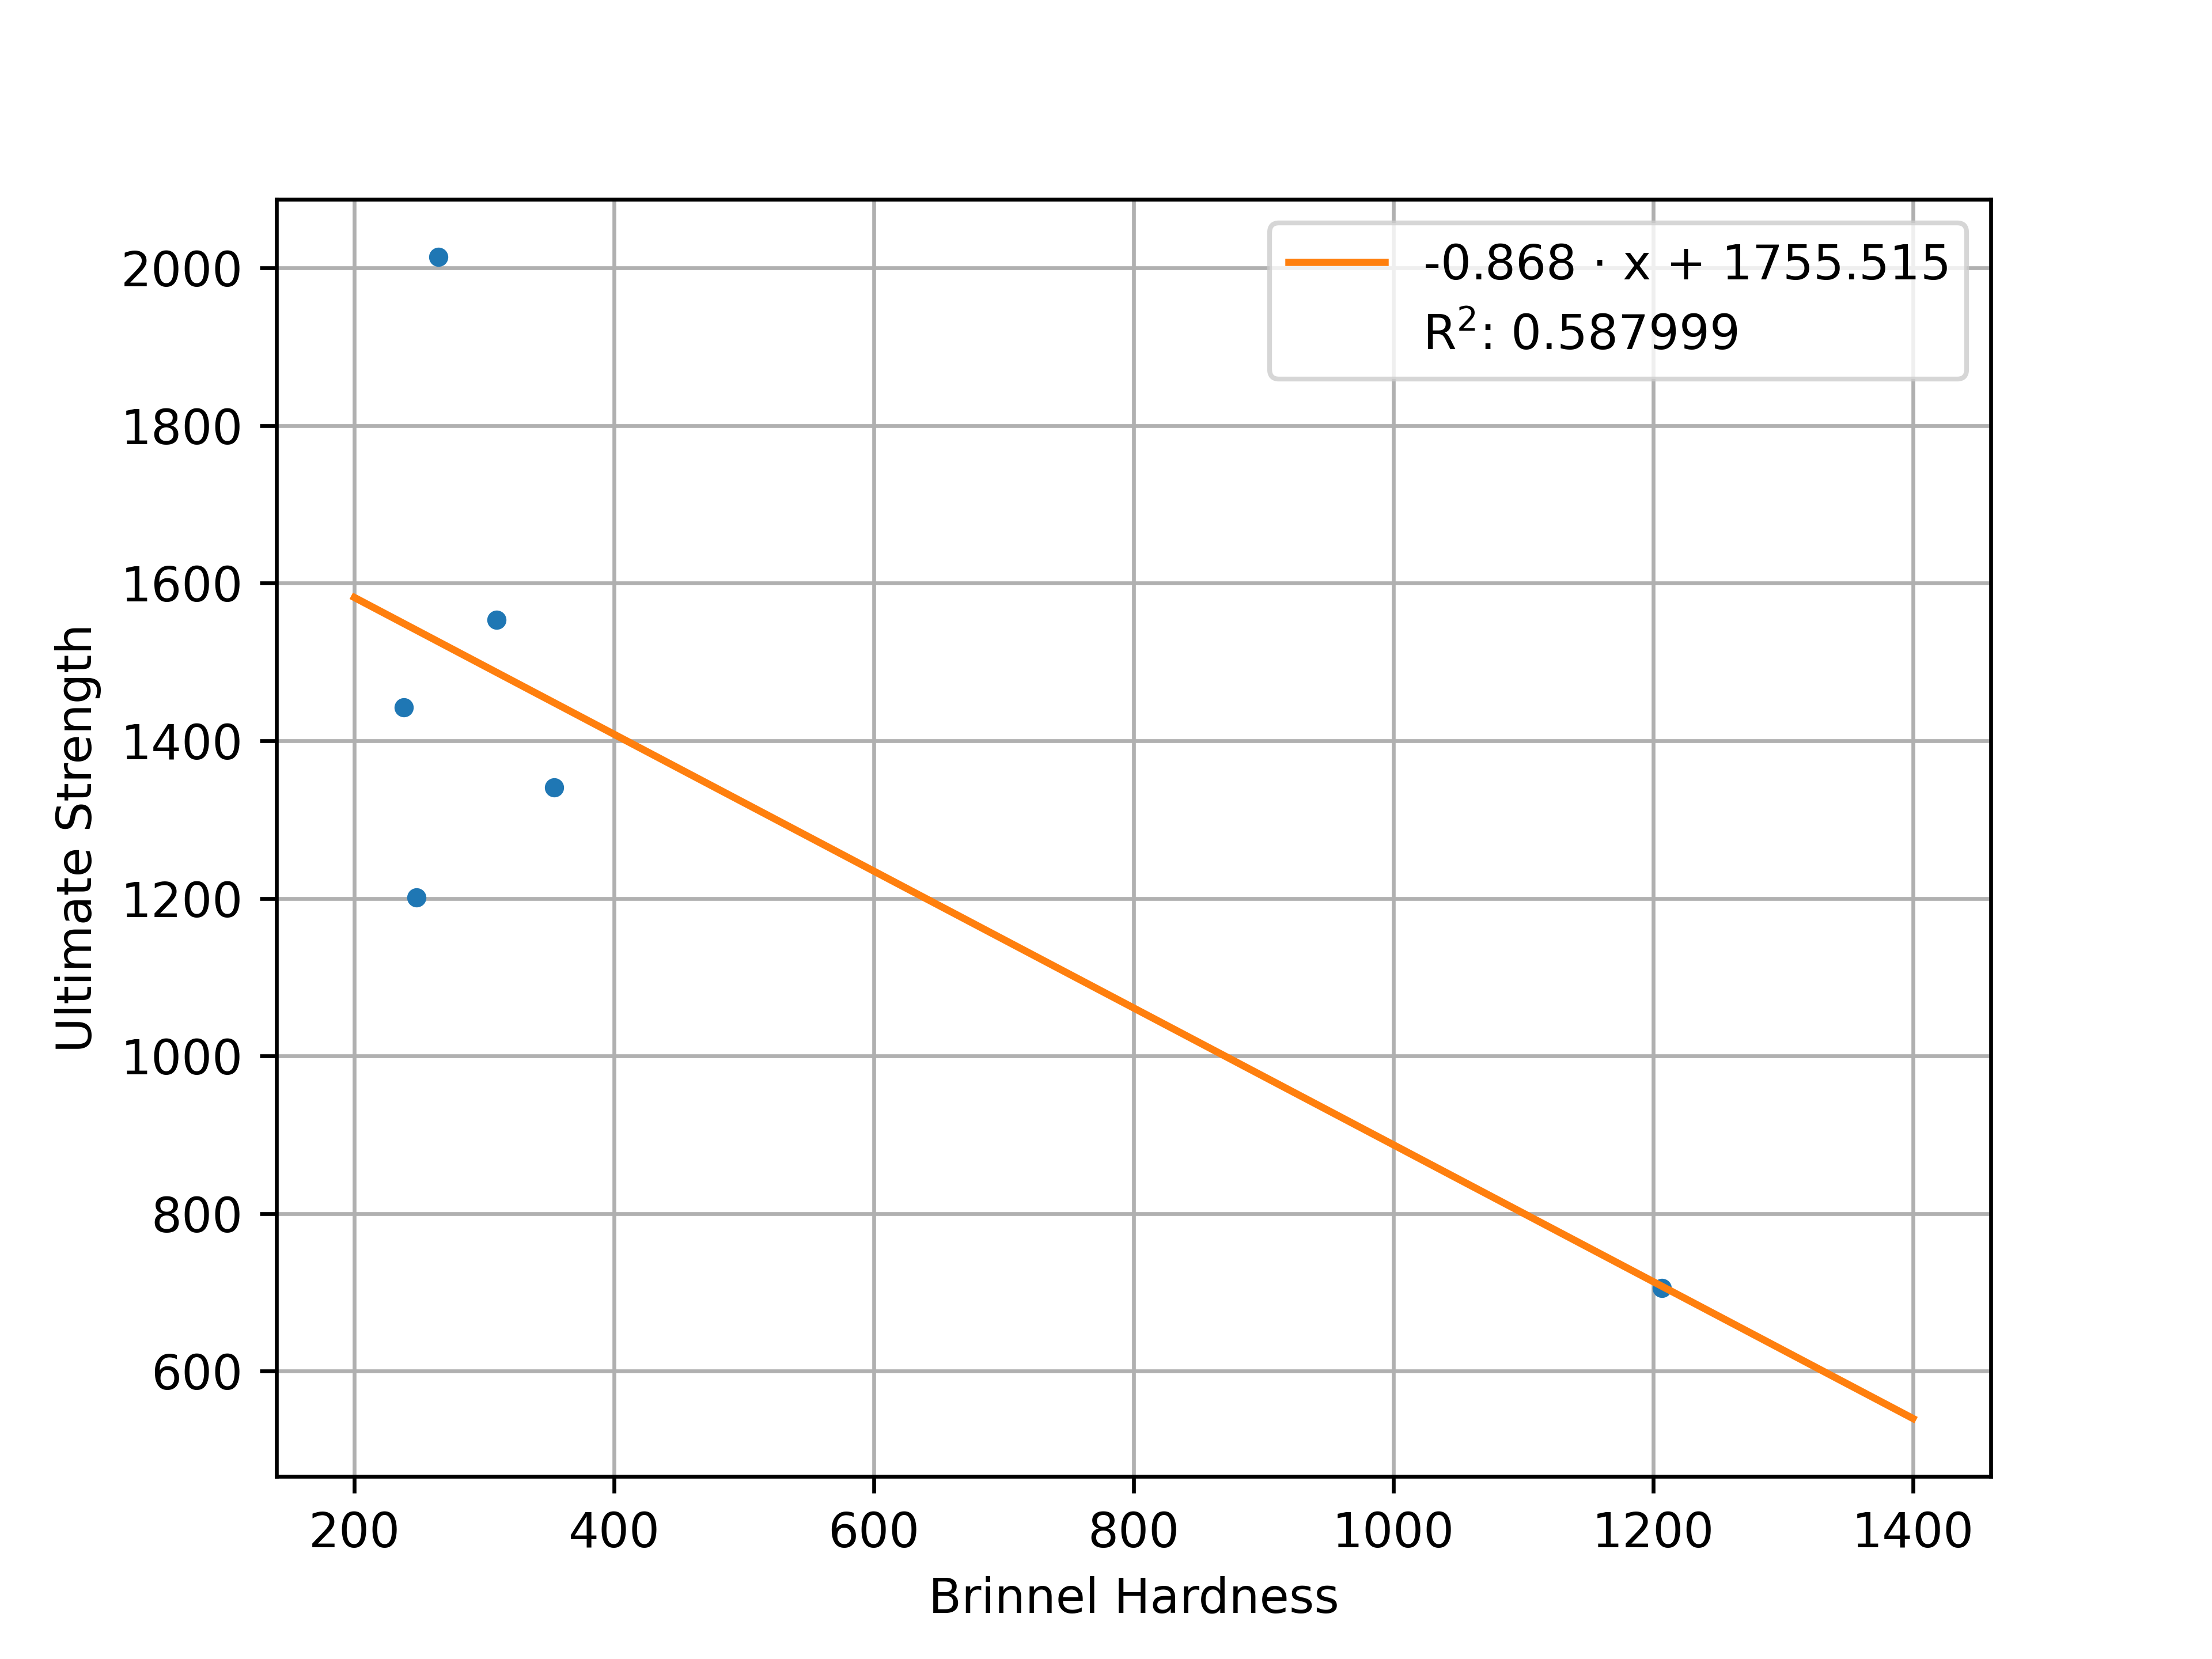
\includegraphics[width=0.5\linewidth]{plots/q4.png}
    \caption{Correlation of $\sigma_{UTS} and HRB$}
    \label{fig:q4}
\end{figure}


\begin{figure}[!h!]
\begin{minipage}[b]{.5\linewidth}
    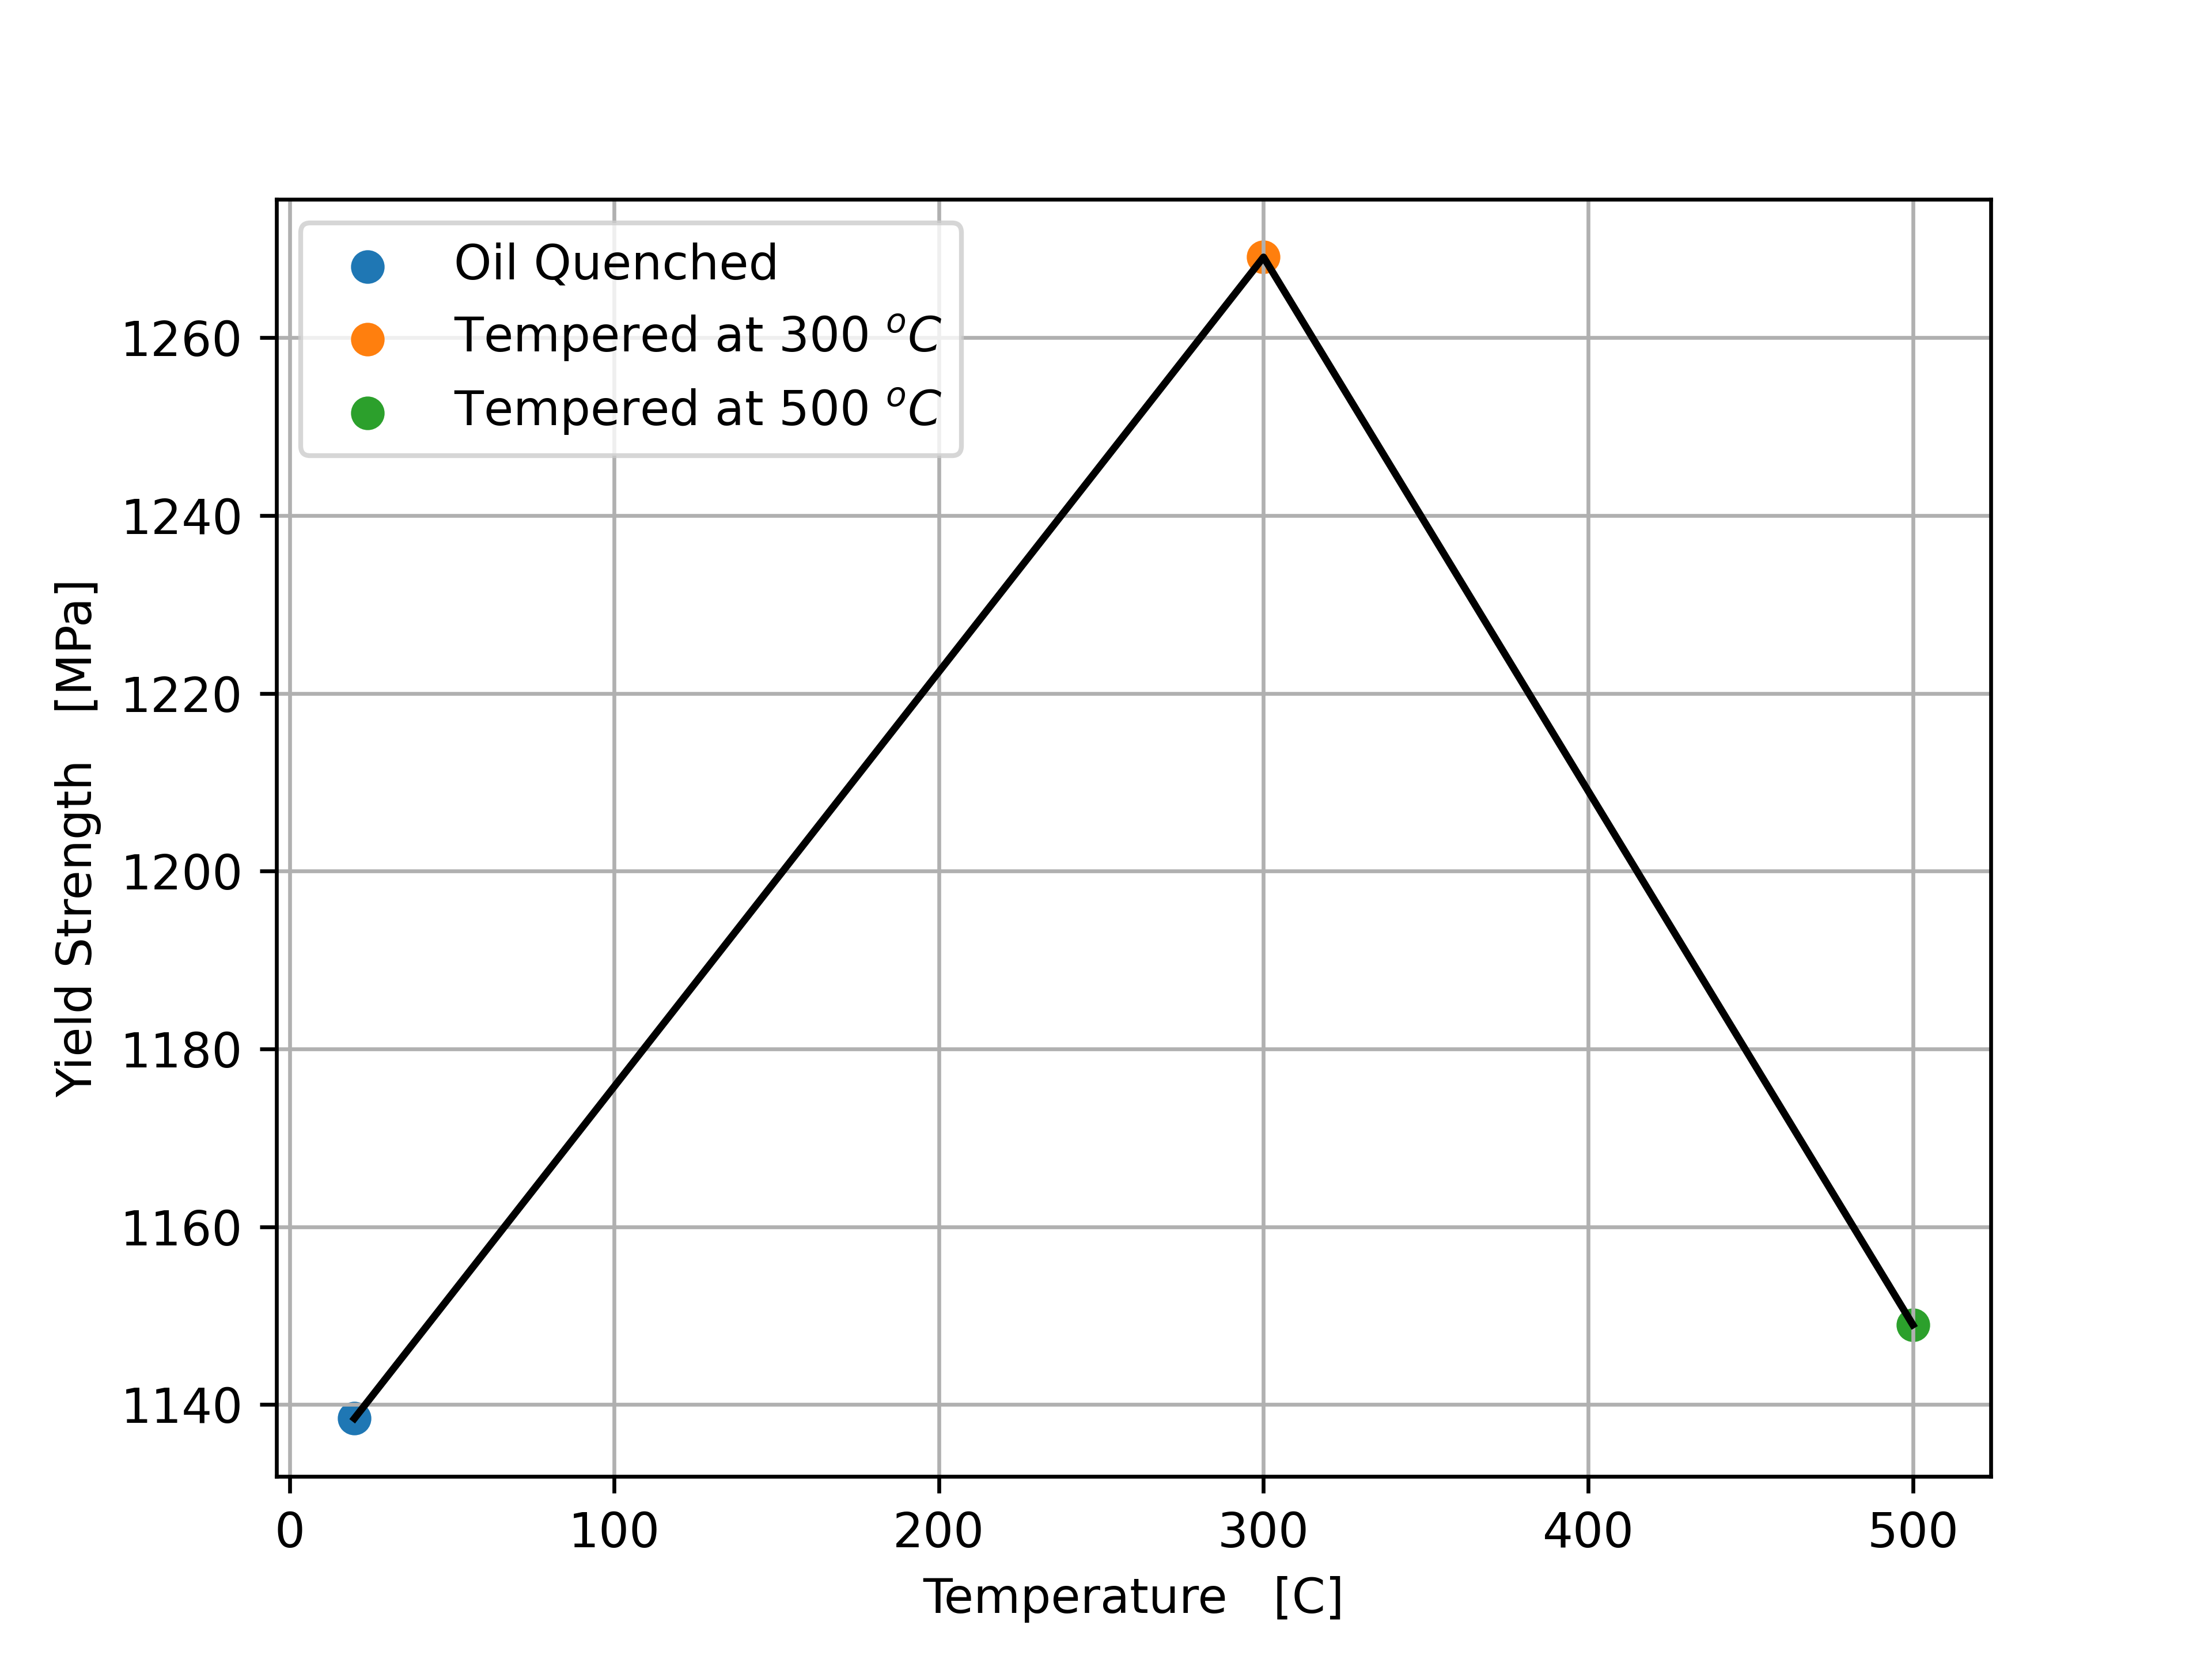
\includegraphics[width=\linewidth]{plots/q6_offset.png}
    \caption{Correlation of $\sigma_y$ to BHN}
    \label{fig:q6-yield}
    \vspace{4ex}
\end{minipage}
\begin{minipage}[b]{.5\linewidth}
    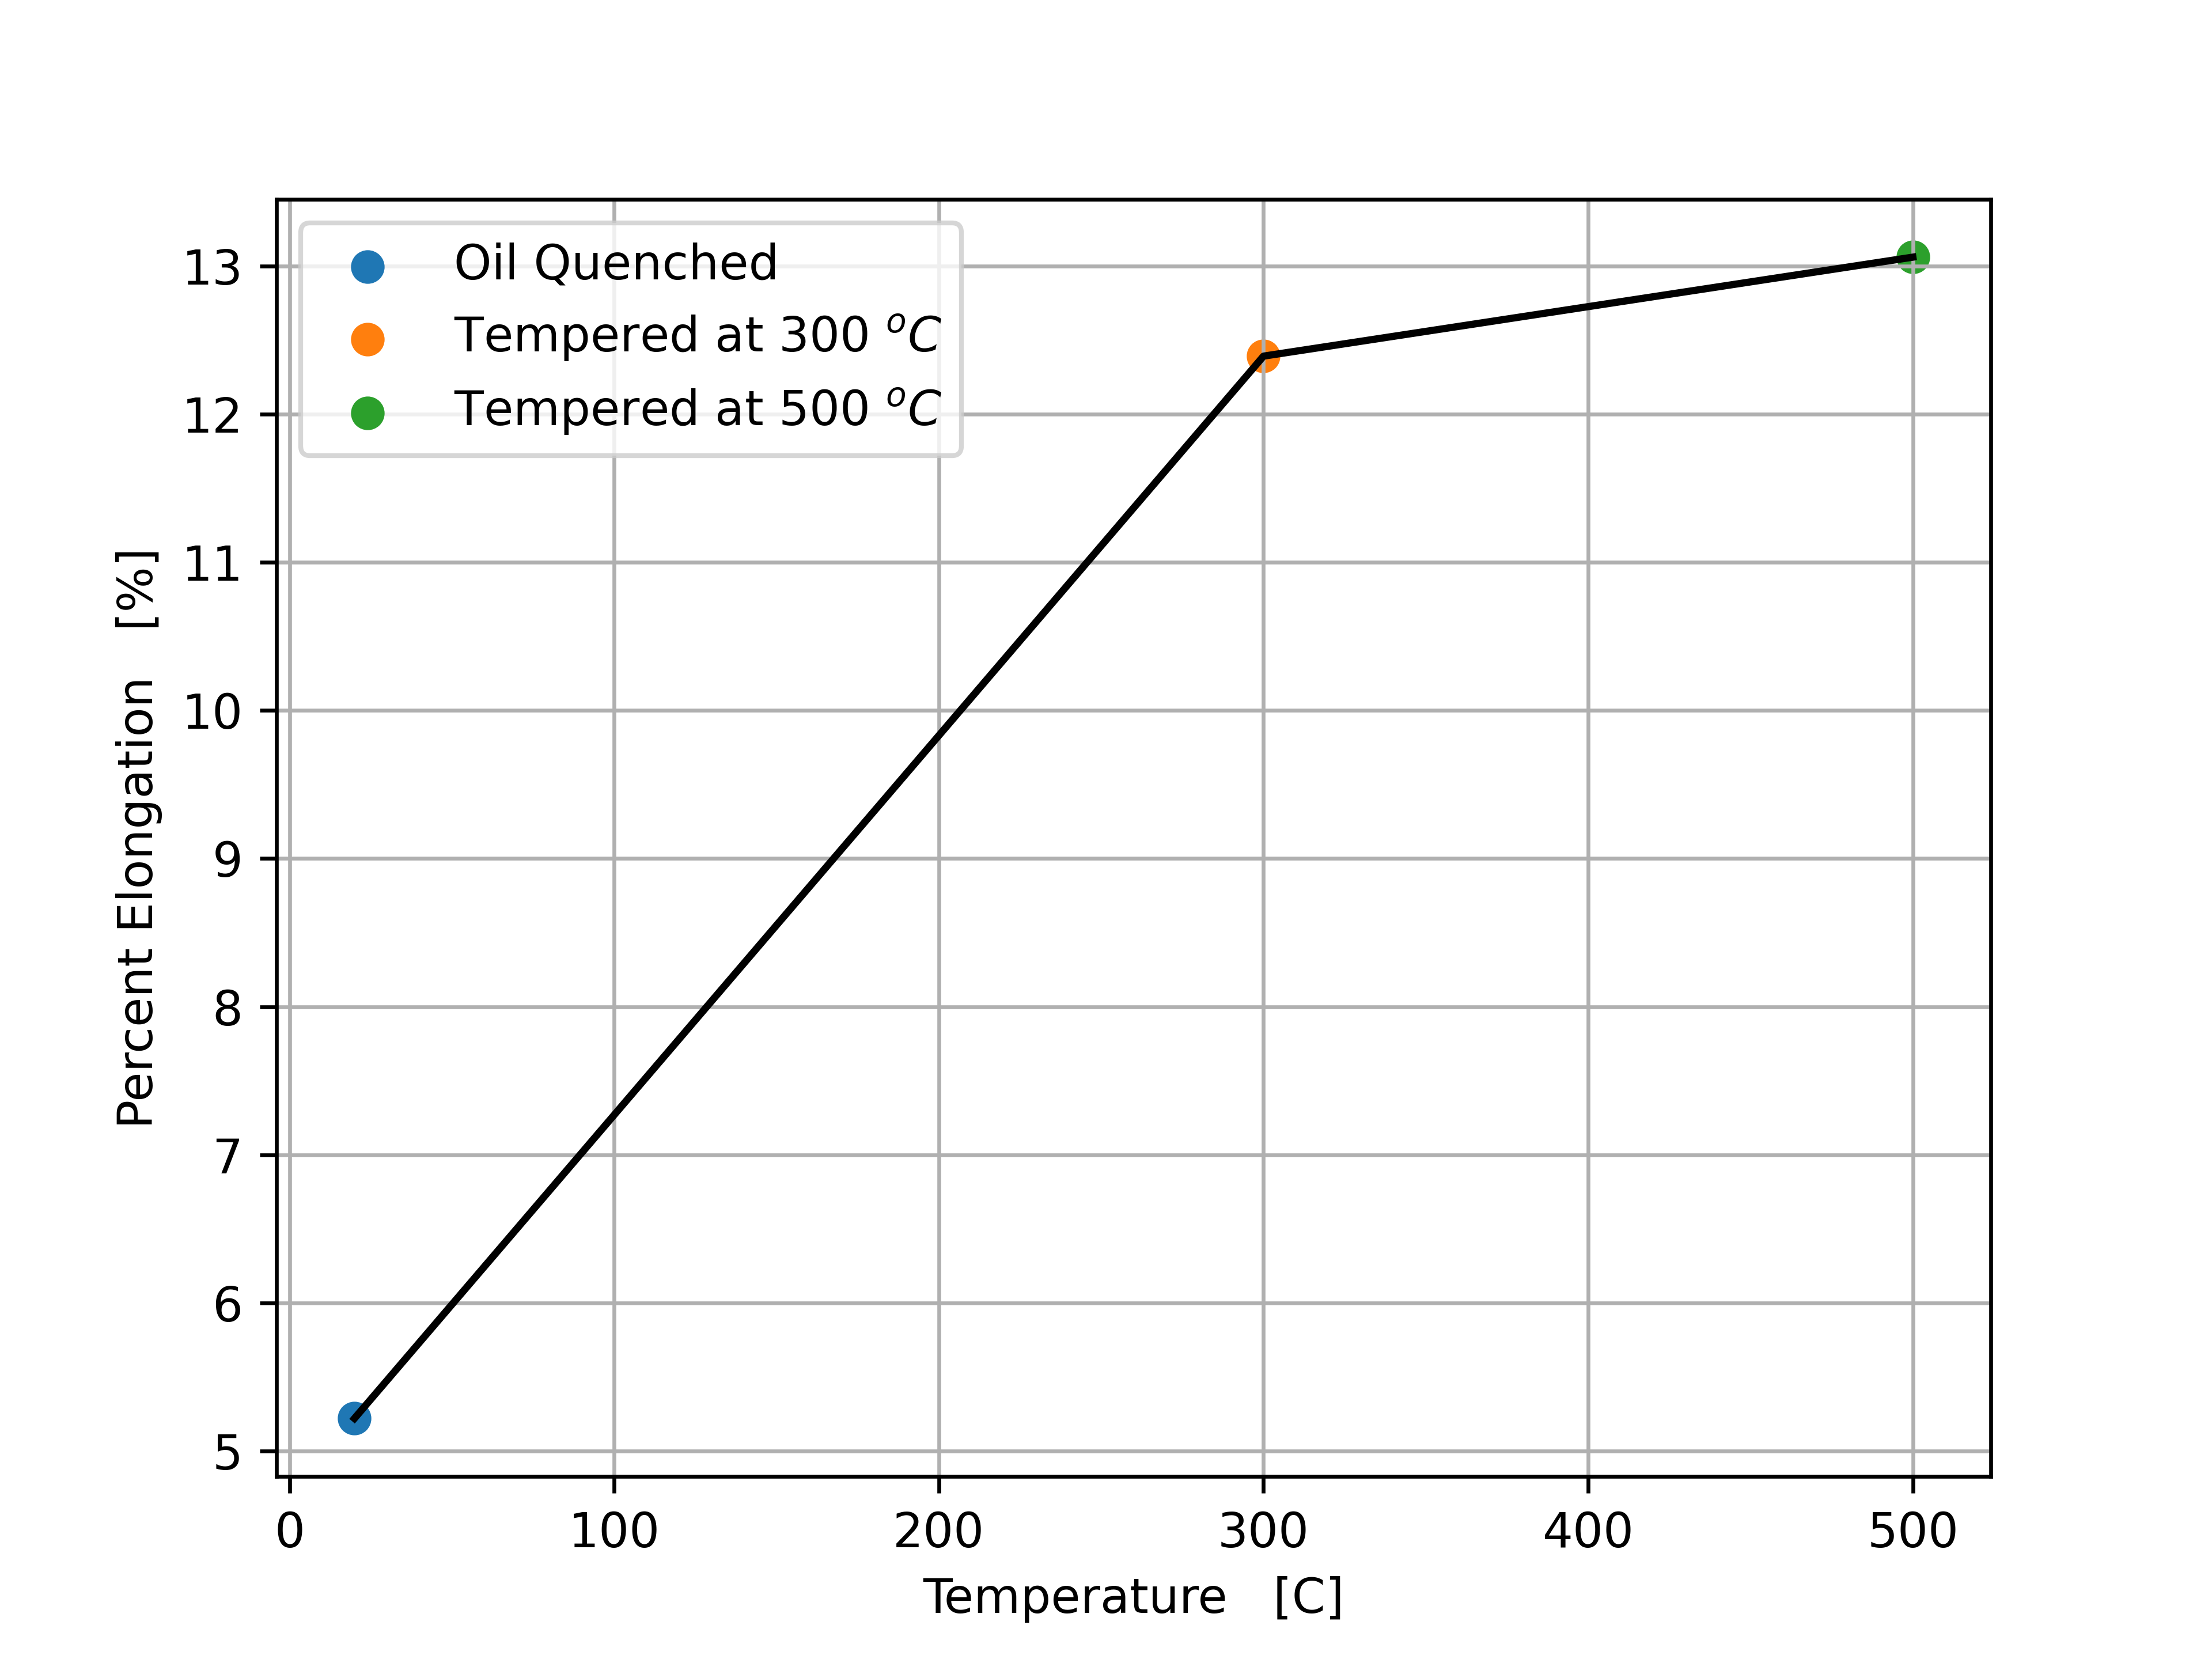
\includegraphics[width=\linewidth]{plots/q6_per_elong.png}
    \caption{Correlation of $\%_{elongation}$ to BHN}
    \label{fig:q6-perelong}
    \vspace{4ex}
\end{minipage}
\begin{minipage}[b]{.5\linewidth}
    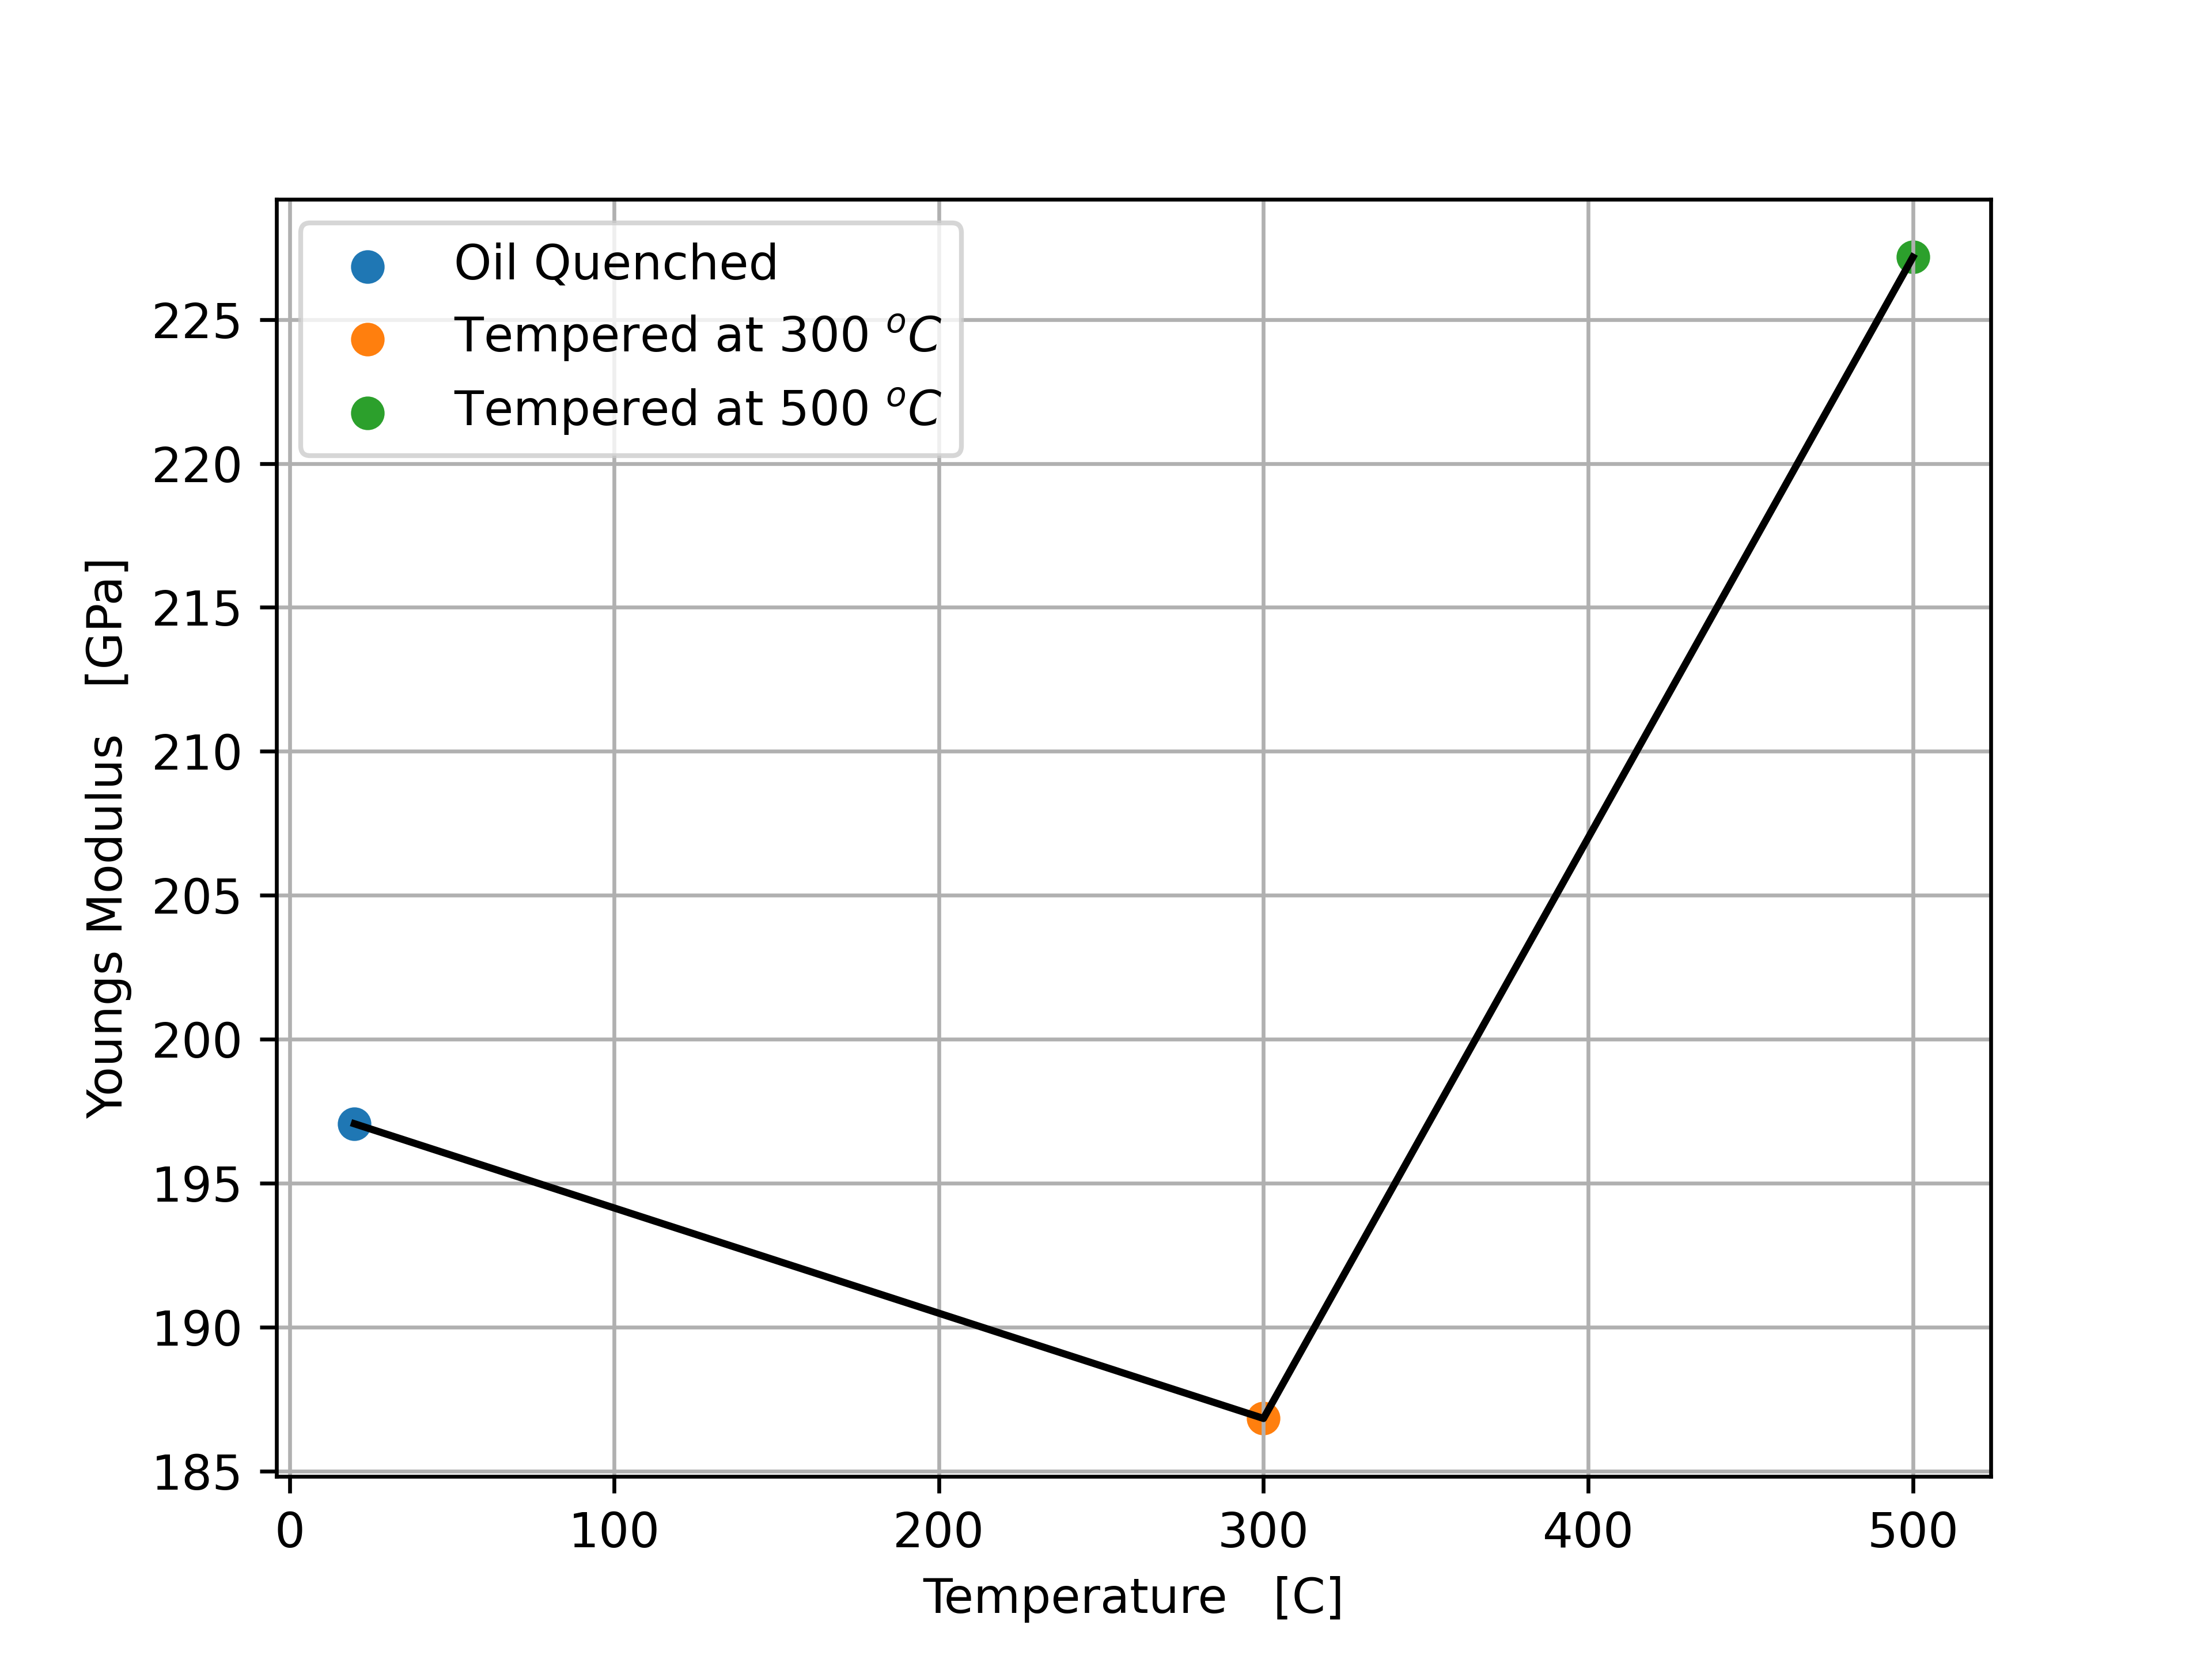
\includegraphics[width=\linewidth]{plots/q6_youngs.png}
    \caption{Correlation of $E$ to BHN}
    \label{fig:q6-youngs}
    \vspace{4ex}
\end{minipage}
\begin{minipage}[b]{.5\linewidth}
    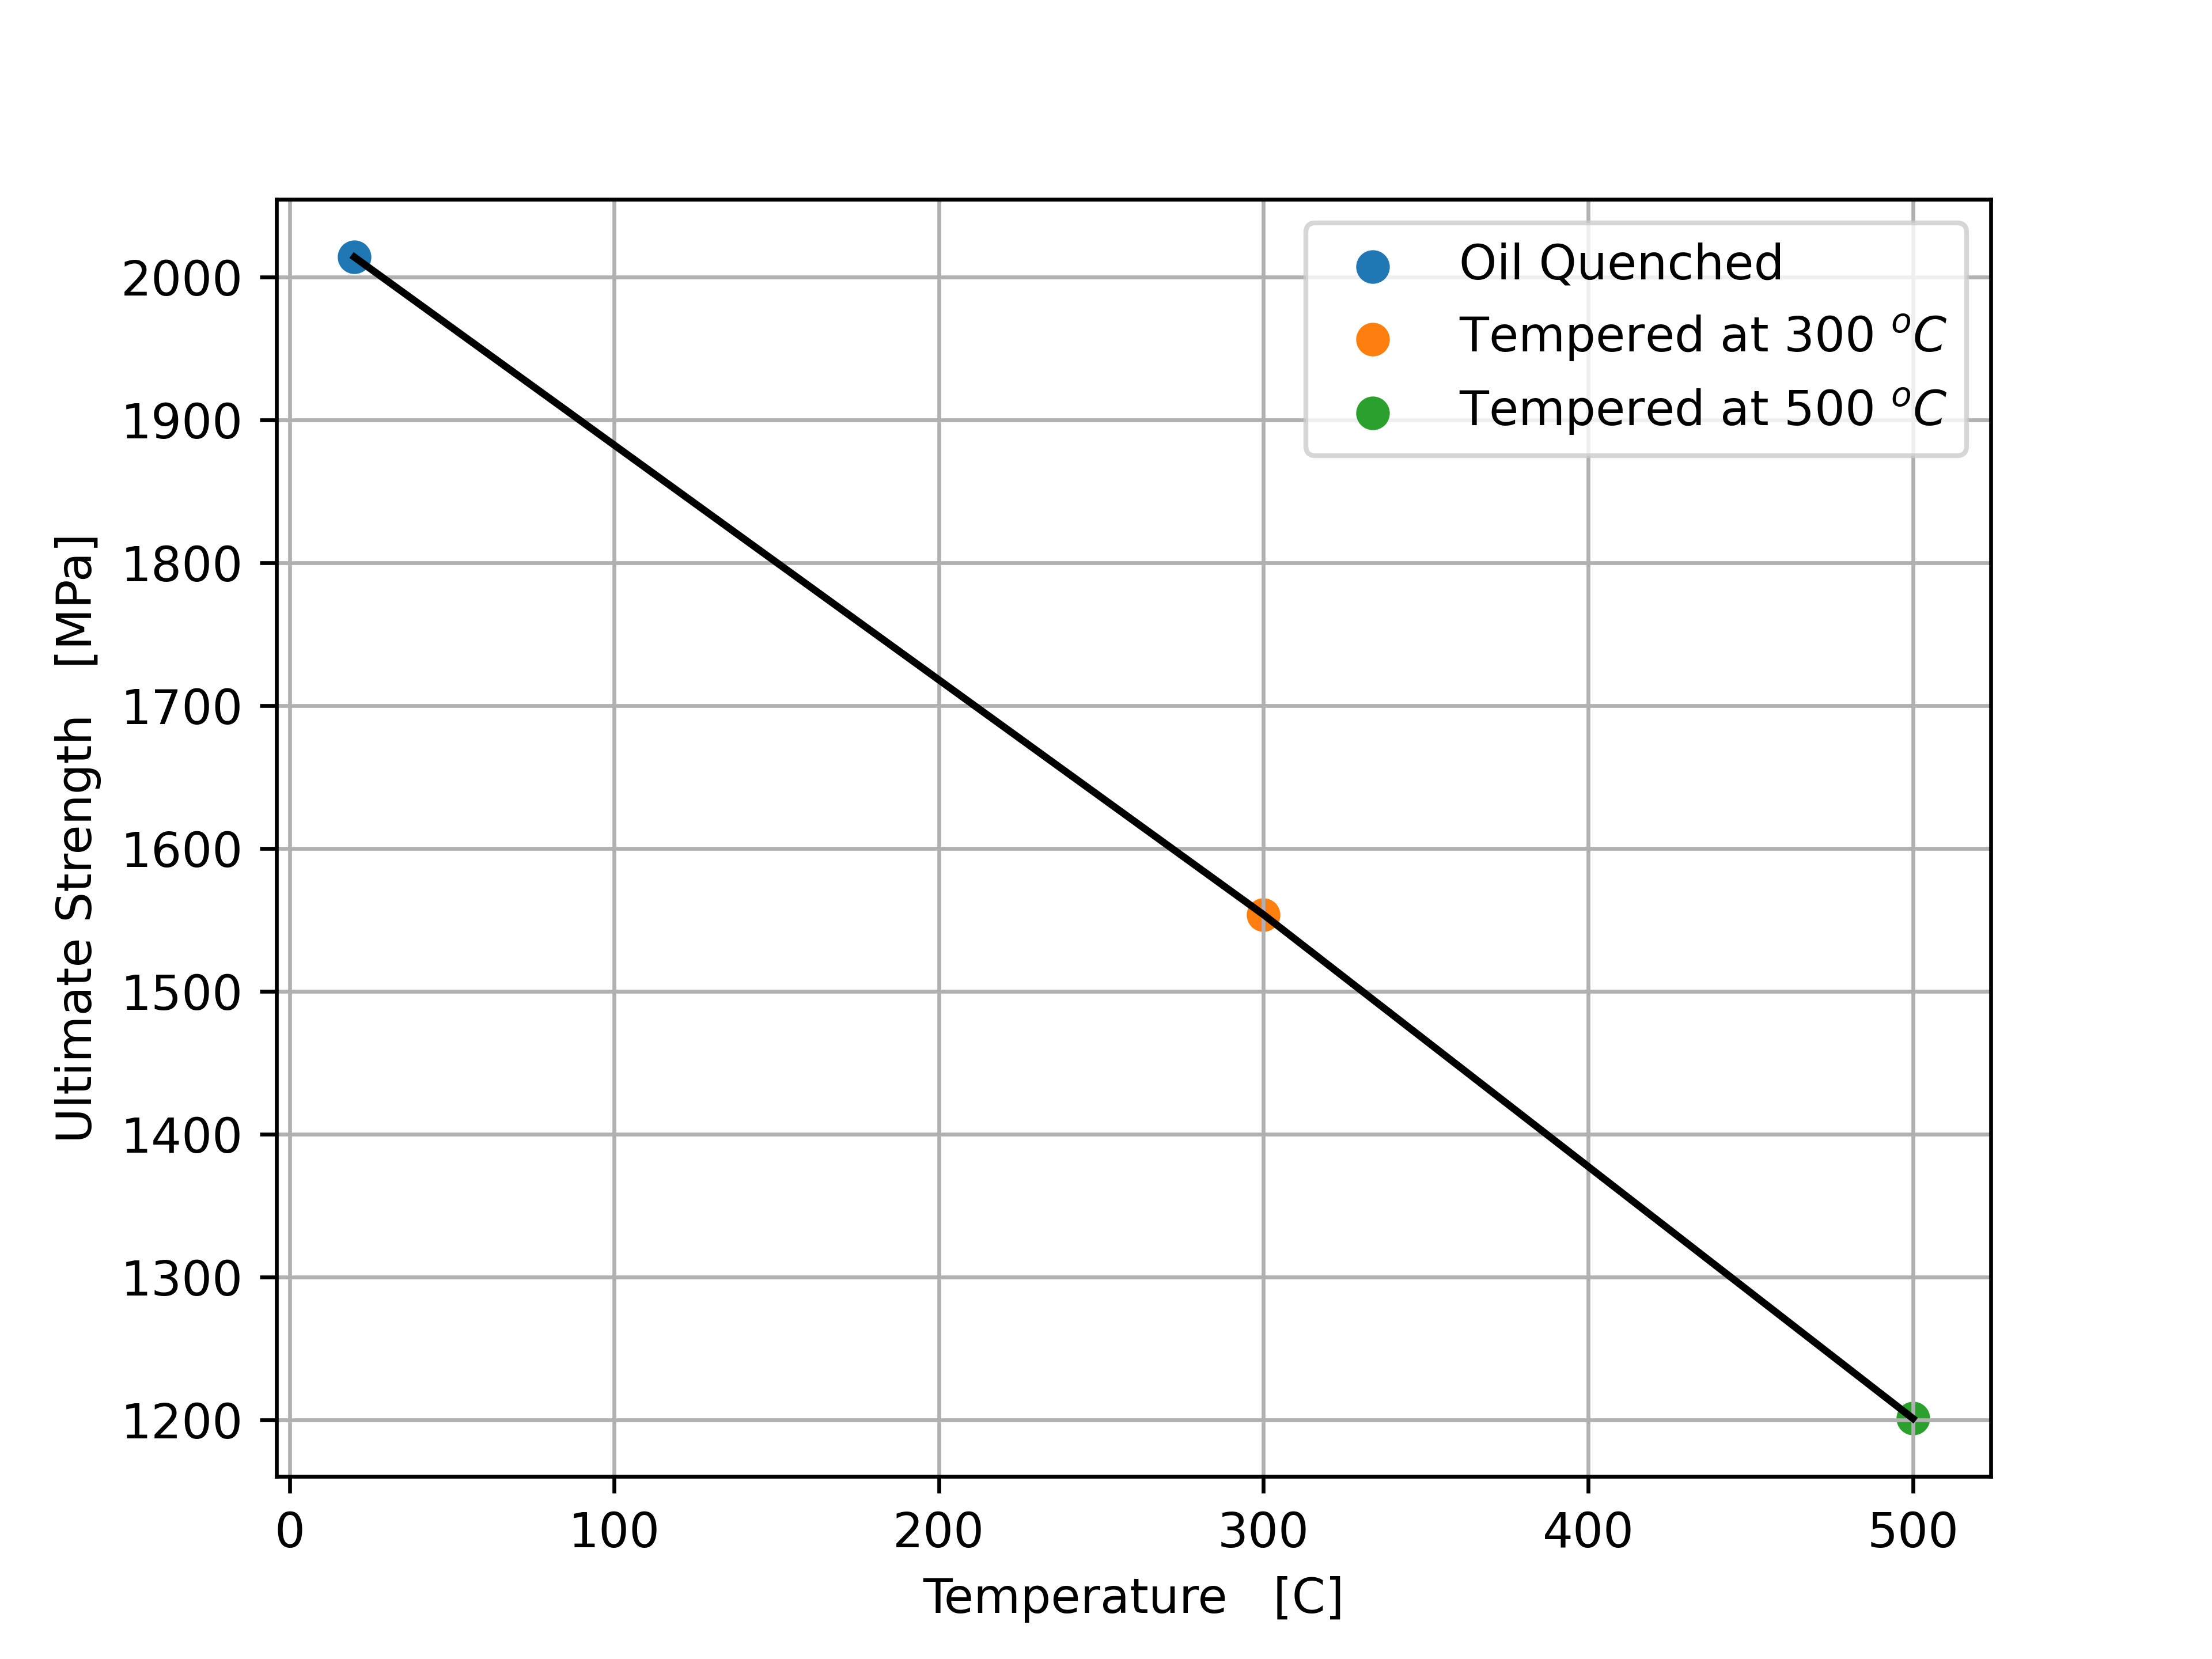
\includegraphics[width=\linewidth]{plots/q6_uts.png}
    \caption{Correlation of $\sigma_{UTS}$ to BHN}
    \label{fig:q6-uts}
    \vspace{4ex}
\end{minipage}
\end{figure}
\newpage
\section{Analysis of Discussion and Results}

\section{Answer to Questions}

\section{Bibliography}

\end{document}